\item La información del cliente que más órdenes haya efectuado. Mostrar el número de órdenes que ha realizado.

\begin{lstlisting}
ordenes = π customerid,orderid (orders)

por_cliente = γ customerid; count(orderid)→total (ordenes)

maximo = γ ; max(total)→mayor (por_cliente)

resultado = σ total = mayor (por_cliente ⨯ maximo)

π customerid,customername,segment,country,city,state,postalcode,region,total (customer ⨝ resultado)
\end{lstlisting}

\begin{center}
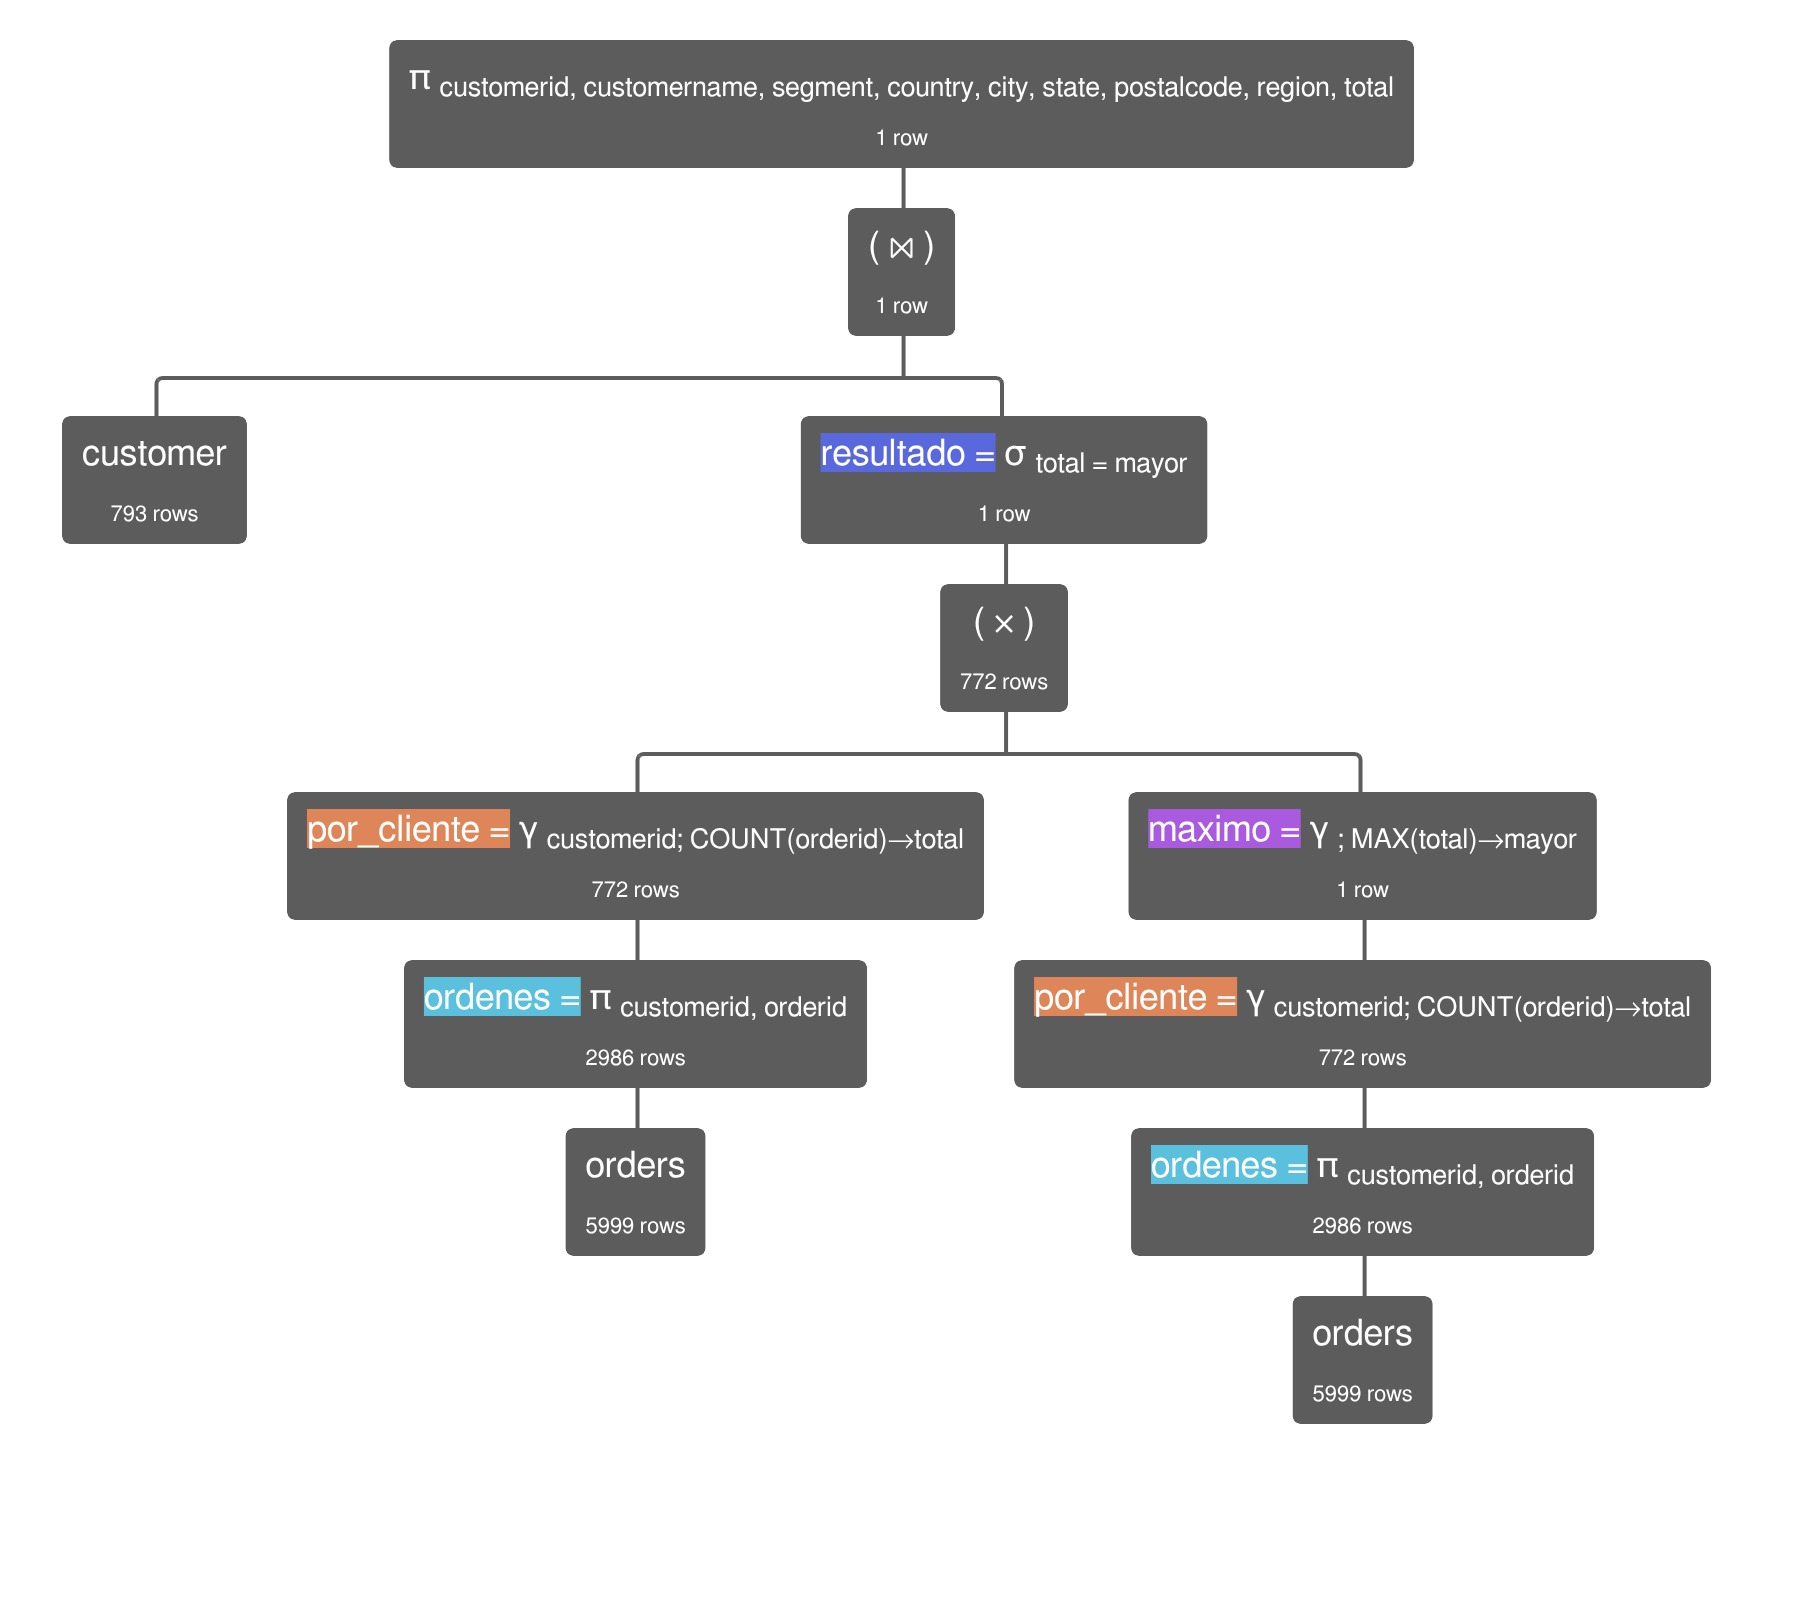
\includegraphics[width=0.75\textwidth]{figuras/2j_1.jpg}
\end{center}

\begin{center}
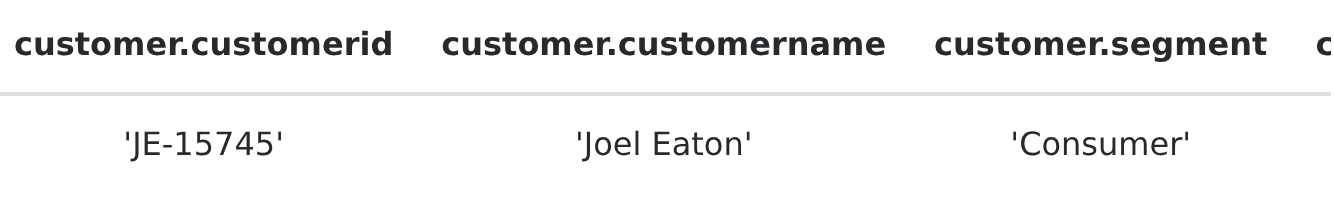
\includegraphics[width=0.4\textwidth]{figuras/2j_2.png}
\end{center}

\newpage
